\documentclass[9pt,a4paper]{report}
\usepackage{amsfonts,amsmath,amsthm,amssymb,graphicx,graphics}
\usepackage{indentfirst,tikz,wrapfig,caption,multirow}
\usepackage[hidelinks]{hyperref}
\usepackage[utf8x]{inputenc}
\renewcommand\figurename{Figura}
\renewcommand\chaptername{Capitolul}
\renewcommand\bibname{Bibliografie}
\newtheorem{definitie}{Definiția}
\newtheorem{teorema}{Teorema}
\newcommand*\nod[1]{\tikz[baseline=(char.base)]{\node[shape=circle,draw,inner sep=1pt] (char) {#1};}}

\begin{document}

\thispagestyle{empty}

\begin{center}
    \bfseries

    \Huge
    INTRODUCERE ÎN \\
    TEORIA GRAFURILOR
    \vspace{25pt}

    \normalsize
    CÂTEVA CONSIDERAȚII ASUPRA CONCEPTELOR \\
    ESENȚIALE CARE STAU LA BAZA TEORIEI GRAFURILOR \\
    ȘI ALGORITMILOR FUNDAMENTALI UTILIZAȚI ÎN \\
    REZOLVAREA PROBLEMELOR COMPUTAȚIONALE \\
    \vspace{25pt}

    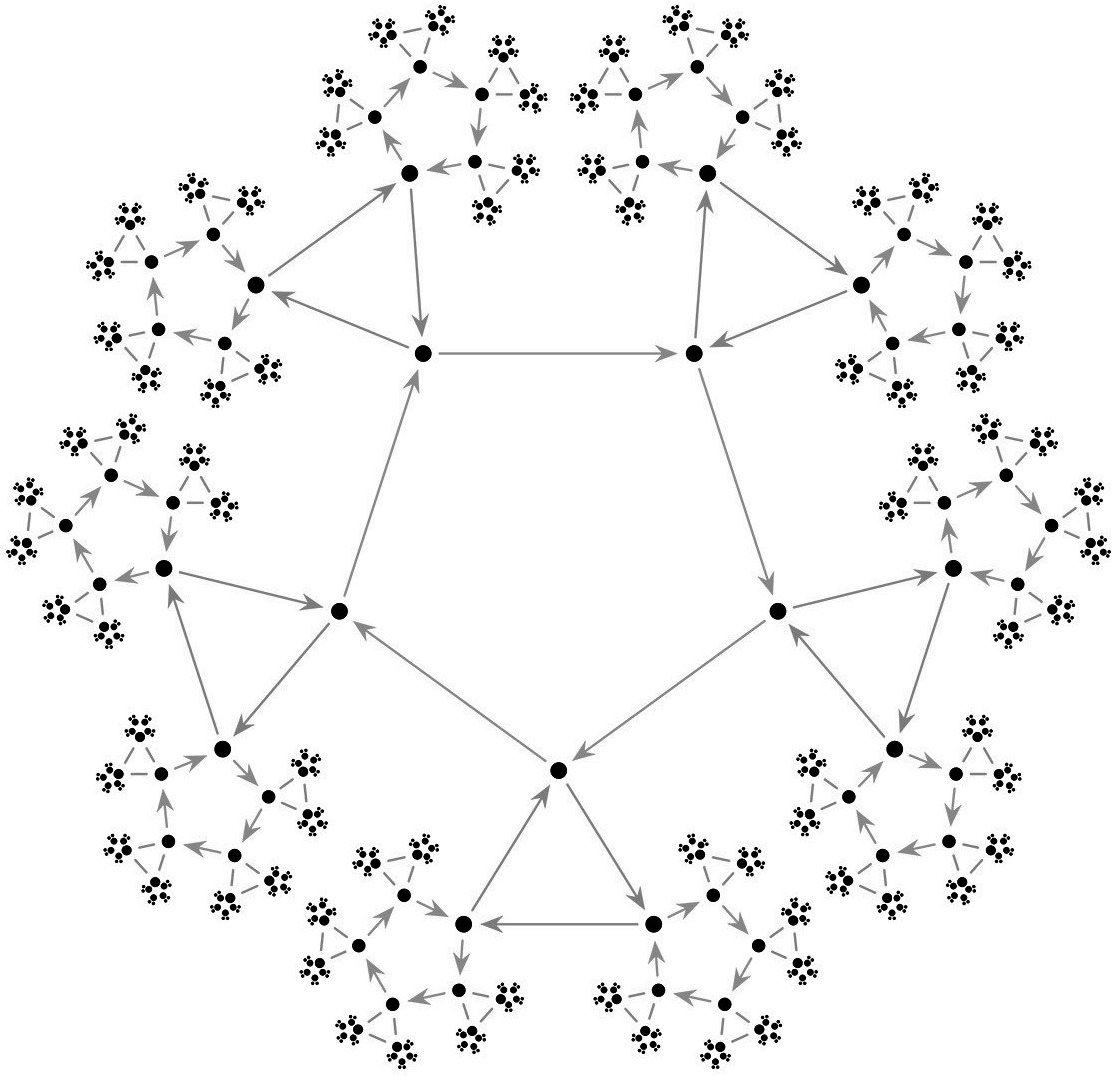
\includegraphics[width=0.9\textwidth]{img/cayley_graph} \\ 
    \textnormal{\textit{Un graf Cayley pentru $C_3 * C_5$.}}
    \vspace{25pt}
    
    \small 
    DE\\
    
    \Large 
    SÎRBU MATEI-DAN \\ 
    \href{mailto:hello@msirbu.eu}{hello@msirbu.eu} \\
    \vspace{25pt}

    BRAȘOV, DECEMBRIE 2020
\end{center}

\newpage
\setcounter{page}{1}

\chapter{Despre conceptul de \textit{graf}}
\section{Terminologie}

Definim în mod informal un graf ca fiind o colecție de ,,noduri'' unite prin ,,muchii'', ca în exemplul următor:

\begin{figure}[htbp]
    \centering
    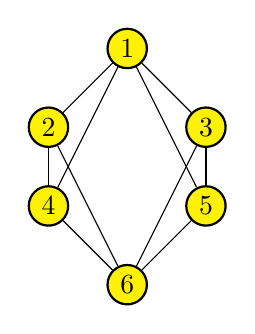
\begin{tikzpicture}[every node/.style={draw=black,thick,circle,inner sep=0pt,fill=yellow,minimum size=0.5cm}]
        \node[] (1) at (0,0) {1};
        \node[] (2) at (-1,-1) {2};
        \node[] (3) at (1,-1) {3};
        \node[] (4) at (-1,-2) {4};
        \node[] (5) at (1,-2) {5};
        \node[] (6) at (0,-3) {6};

        \path [-] (1) edge (3);
        \path [-] (1) edge (4);
        \path [-] (1) edge (5);
        \path [-] (2) edge (4);
        \path [-] (1) edge (2);
        \path [-] (2) edge (6);
        \path [-] (3) edge (5);
        \path [-] (3) edge (6);
        \path [-] (4) edge (6);
        \path [-] (5) edge (6);
    \end{tikzpicture}
    \caption{Un graf neorientat oarecare.}
    \label{fig:graf1}
\end{figure}

\begin{definitie}
    Un \textbf{graf} este o pereche $(V,E)$, unde $V$ este o mulțime finită de elemente, numite \textit{noduri (\textbf{V}ertices)}, iar $E$ este o mulțime finită de perechi de noduri, numite \textit{muchii (\textbf{E}dges)}.
\end{definitie}

Dacă perechile din mulțimea $E$ sunt ordonate, atunci spunem că graful este \textbf{\textit{orientat}}, sau \textbf{\textit{digraf}}; în caz contrar, graful este \textbf{\textit{neorientat}}. De asemenea, două noduri unite de o muchie se numesc \textit{\textbf{adiacente}}. Conceptul analog muchiilor aplicabil grafurilor orientate este \textbf{\textit{arcul}}.

\section{Dimensiunile unui graf}

De obicei, notăm cu $n$ numărul de noduri ale unui graf; mai precis, $n = |V|$. Cu $m$ vom nota numărul de muchii, adică $m = |E|$. În graful din figura \ref{fig:graf1}, $n$ este 6, iar $m$ este 10.

\begin{teorema}
    Dacă un graf neorientat are $n$ noduri, atunci \textbf{\textit{numărul total de grafuri neorientate}}\textsuperscript{\cite{milosescu}} care se pot forma cu aceste noduri este $g = 2^{C_n^2}$.
\end{teorema}

\begin{teorema}
    Graful \textbf{\textit{complet}}, graful care are toate muchiile posibile, conține $m = \frac{n(n-1)}{2}$ muchii, dacă este neorientat.
\end{teorema}

Spunem despre un nod că este \textbf{\textit{izolat}} dacă nu aparține niciunei muchii. Întrucât nodurile izolate sunt inutile în majoritatea aplicațiilor, presupunem că nu există astfel de noduri; în acest caz, știm despre numărul de muchii că este $m \geq \frac{n}{2}$.

Astfel, deducem, utilizând simbolul O al lui Landau (notația \textit{big-O}), că în general, $m = O(n^2)$, iar în majoritatea aplicațiilor, $m = \Omega(n)$, limite care sunt aplicabile și digrafurilor. Din punct de vedere terminologic, grafurile cu $m = \Theta(n)$ se numesc \textbf{\textit{rare}}, iar cele cu $m = \Theta(n^2)$ sunt \textbf{\textit{dense}}\textsuperscript{\cite{gabow}}.

\section{Conexitate}

\begin{definitie}
    Un \textbf{subgraf} $G' = (V', E')$ este un subgraf al lui $G = (V, E)$ dacă $V' \subseteq V$ și $E' \subseteq E$.
\end{definitie}
\begin{definitie}
    Un \textbf{lanț} este o succesiune de noduri $v_0, v_1, \dots, v_l$, $l \geq 0$, cu $(v_i, v_{i+1}) \in E$ pentru $i = \overline{0, \ l - 1}$. Analog, în cazul grafurilor orientate, această succesiune de noduri se numește \textbf{drum}.
\end{definitie}

Un lanț este \textbf{\textit{simplu}} dacă nu trece de două ori prin aceeași muchie. În caz contrar, se numește lanț \textbf{\textit{compus}}. Este de remarcat faptul că un lanț poate avea lungime nulă.

\begin{definitie}
    Un \textbf{ciclu} este un drum cu $l \geq 3$, $v_0 = v_l$ cu toate nodurile și muchiile distincte.
\end{definitie}

\begin{definitie}
    \textbf{Gradul} unui nod $v_k$ al grafului $G$ este egal cu numărul muchiilor incidente cu nodul și se notează cu $d(v_k)$.
\end{definitie}

În funcție de gradul nodurilor putem distinge câteva cazuri particulare\textsuperscript{\cite{milosescu}}. Un \textbf{\textit{nod terminal}} este incident cu o singură muchie, adică $d(v_k) = 1$. Un \textbf{\textit{nod izolat}} nu este adiacent cu nici un alt nod al grafului, adică nu se găsește în extremitatea niciunei muchii; altfel spus, $d(v_k) = 0$. Un exemplu\textsuperscript{\cite{milosescu}}:

\begin{center}
    \begin{minipage}[t]{0.5\textwidth}
        \vspace{0pt} % force top alignment when using text and figure
        Graful $G = (V, E)$ din figură este definit astfel:
        \begin{itemize}
            \item $V = \{1, 2, 3, \dots, 11\}$
            \item $E = \{(1,2), (1,4), (2,3), (2,5), \\ (3,4), (3,5), (5,6), (5,7), (5,8), (7,9)\}$
        \end{itemize}
        Despre graful $G$ putem spune că:
    \end{minipage}
    \begin{minipage}[t]{0.49\textwidth}
        \vspace{0pt}
        \begin{flushright}
            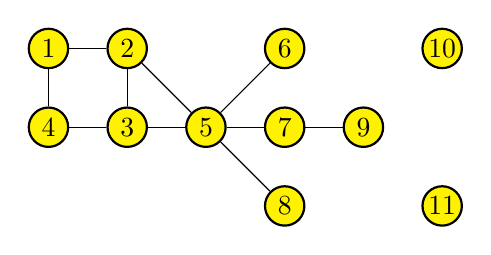
\begin{tikzpicture}[every node/.style={draw=black,thick,circle,inner sep=0pt,fill=yellow,minimum size=0.5cm}]
                \node[] (1) at (0,0) {1};
                \node[] (2) at (1,0) {2};
                \node[] (3) at (1,-1) {3};
                \node[] (4) at (0,-1) {4};
                \node[] (5) at (2,-1) {5};
                \node[] (6) at (3,0) {6};
                \node[] (7) at (3,-1) {7};
                \node[] (8) at (3,-2) {8};
                \node[] (9) at (4,-1) {9};
                \node[] (10) at (5,0) {10};
                \node[] (11) at (5,-2) {11};

                \path [-] (1) edge (2);
                \path [-] (1) edge (4);
                \path [-] (2) edge (3);
                \path [-] (2) edge (5);
                \path [-] (3) edge (4);
                \path [-] (3) edge (5);
                \path [-] (5) edge (6);
                \path [-] (5) edge (7);
                \path [-] (5) edge (8);
                \path [-] (7) edge (9);
            \end{tikzpicture}
        \end{flushright}
    \end{minipage}
\end{center}

\begin{itemize}
    \item $d(v_5) = 5$, deoarece \nod{5} are 5 muchii incidente: $(2,5), (3,5), (5,6), (5,7)$ și $(5,8)$.
    \item $d(v_9) = 1$, adică \nod{9} este \textit{nod terminal}, deoarece are o singură muchie incidentă: $(7,9)$.
    \item $d(v_{10}) = 0$, adică \nod{10} este \textit{nod izolat}, deoarece nu are muchii incidente.
\end{itemize}

\begin{thebibliography}{9}
    \bibitem{gabow}
    Harold N. Gabow.
    \href{https://www.cs.colorado.edu/~hal/Papers/DFS/alldfs.pdf}{\textit{Graph Theory Definitions}}.
    The Department of Computer Science at the University of Colorado Boulder, 2008.

    \bibitem{milosescu}
    Mariana Miloșescu.
    \textit{Informatică intensiv: C++: manual pentru clasa a XI-a, ed. a 3-a}.
    Editura Didactică și Pedagogică, 2012.
\end{thebibliography}

\end{document}